% ============================================================
%  chapter2_requirements_methodology.tex
% ============================================================
\chapter[Requirements and Methodology]{Requirements Analysis, Specifications and Methodology}
\label{ch:requirements}

This chapter translates the gaps identified in Chapter~\ref{ch:state-of-the-art} into
a verifiable specification for the Knowledge Platform. It analyses the host-organisation
context, defines functional and non-functional requirements with acceptance criteria,
and establishes the Agile Scrum methodology and five-sprint delivery plan that
structure the design (Chapter~\ref{ch:architecture}), implementation
(Chapter~\ref{ch:implementation}), and validation (Chapter~\ref{ch:validation})
chapters.

\section{Analysis of the Existing Situation and Usage Context}

\subsection{Host Organisation Context}

\textbf{\CompanyName} is a technology company whose teams produce and consume
significant volumes of internal documentation: technical specifications, onboarding
guides, project reports, API references, and operational procedures. Prior to this
project, knowledge was distributed across disconnected tools — shared drives, email
threads, and informal messaging channels — with no unified governance model and no
mechanism for intelligent retrieval.

The key pain points identified through analysis of the existing situation were:

\begin{itemize}
  \item \textbf{Fragmented storage}: documents resided in multiple systems with no
    single point of access, making comprehensive search impossible.
  \item \textbf{No access governance}: there was no systematic control over which
    teams or roles could access which documents, leading to either over-sharing or
    information silos.
  \item \textbf{Keyword-only search}: retrieval was limited to filename and keyword
    matching, returning documents rather than answers.
  \item \textbf{Onboarding friction}: new employees had no reliable way to find answers
    to operational questions, creating repeated interruptions to experienced colleagues.
  \item \textbf{No feedback mechanism}: when information found through search was
    incorrect or outdated, there was no way to signal this or prevent the same error
    from recurring.
\end{itemize}

\subsection{System Actors}

Four actor groups interact with the Knowledge Platform, as summarized in
Table~\ref{tab:actors} and detailed in the global use-case diagram
(Subsection~\ref{subsec:global-use-case}, Figure~\ref{fig:use-cases}):

\begin{table}[H]
\centering
\caption{System actors and their primary capabilities}
\label{tab:actors}
\renewcommand{\arraystretch}{1.4}
\begin{tabularx}{\textwidth}{|>{\RaggedRight\arraybackslash}p{2.8cm}|Y|}
\hline
\rowcolor{sectionblue!15}
\textbf{Actor} & \textbf{Primary capabilities} \\
\hline
\textbf{Employee} &
Browse and search the document library, perform semantic search and RAG
question-answering, manage personal profile, maintain conversation history,
and rate assistant answers. \\
\hline
\textbf{Manager} &
All Employee capabilities, plus access to the manager dashboard showing
managed departments and their members, and the ability to send announcements
to managed departments. \\
\hline
\textbf{Administrator} &
Full platform control: user lifecycle management, department CRUD and merge,
per-user restrictions, bulk operations, audit log access, KPI dashboards,
activity exports, and platform-wide notifications. \\
\hline
\textbf{System} &
Autonomous actor: executes the BullMQ ingest worker (extract, chunk, embed),
emits automatic notifications on document and role events, and runs the RAG
evaluation harness. \\
\hline
\end{tabularx}
\end{table}

\subsection{Global Use-Case Model}
\label{subsec:global-use-case}

Figure~\ref{fig:use-cases} presents the global use-case model of the Knowledge
Platform. It identifies primary actors (\textbf{Guest}, \textbf{Employee},
\textbf{Manager}, and \textbf{Administrator}), with the three authenticated roles
generalizing an abstract \textbf{Authenticated user} actor. Use cases are grouped
into authentication, document management, search and AI, notifications, and
governance domains. Secondary actors (\textbf{Email}, \textbf{Gemini}, and
\textbf{BullMQ worker}) model external interactions through
\texttt{<<notify>>}, \texttt{<<invoke>>}, and \texttt{<<enqueue>>} dependencies.

\begin{figure}[H]
  \centering
  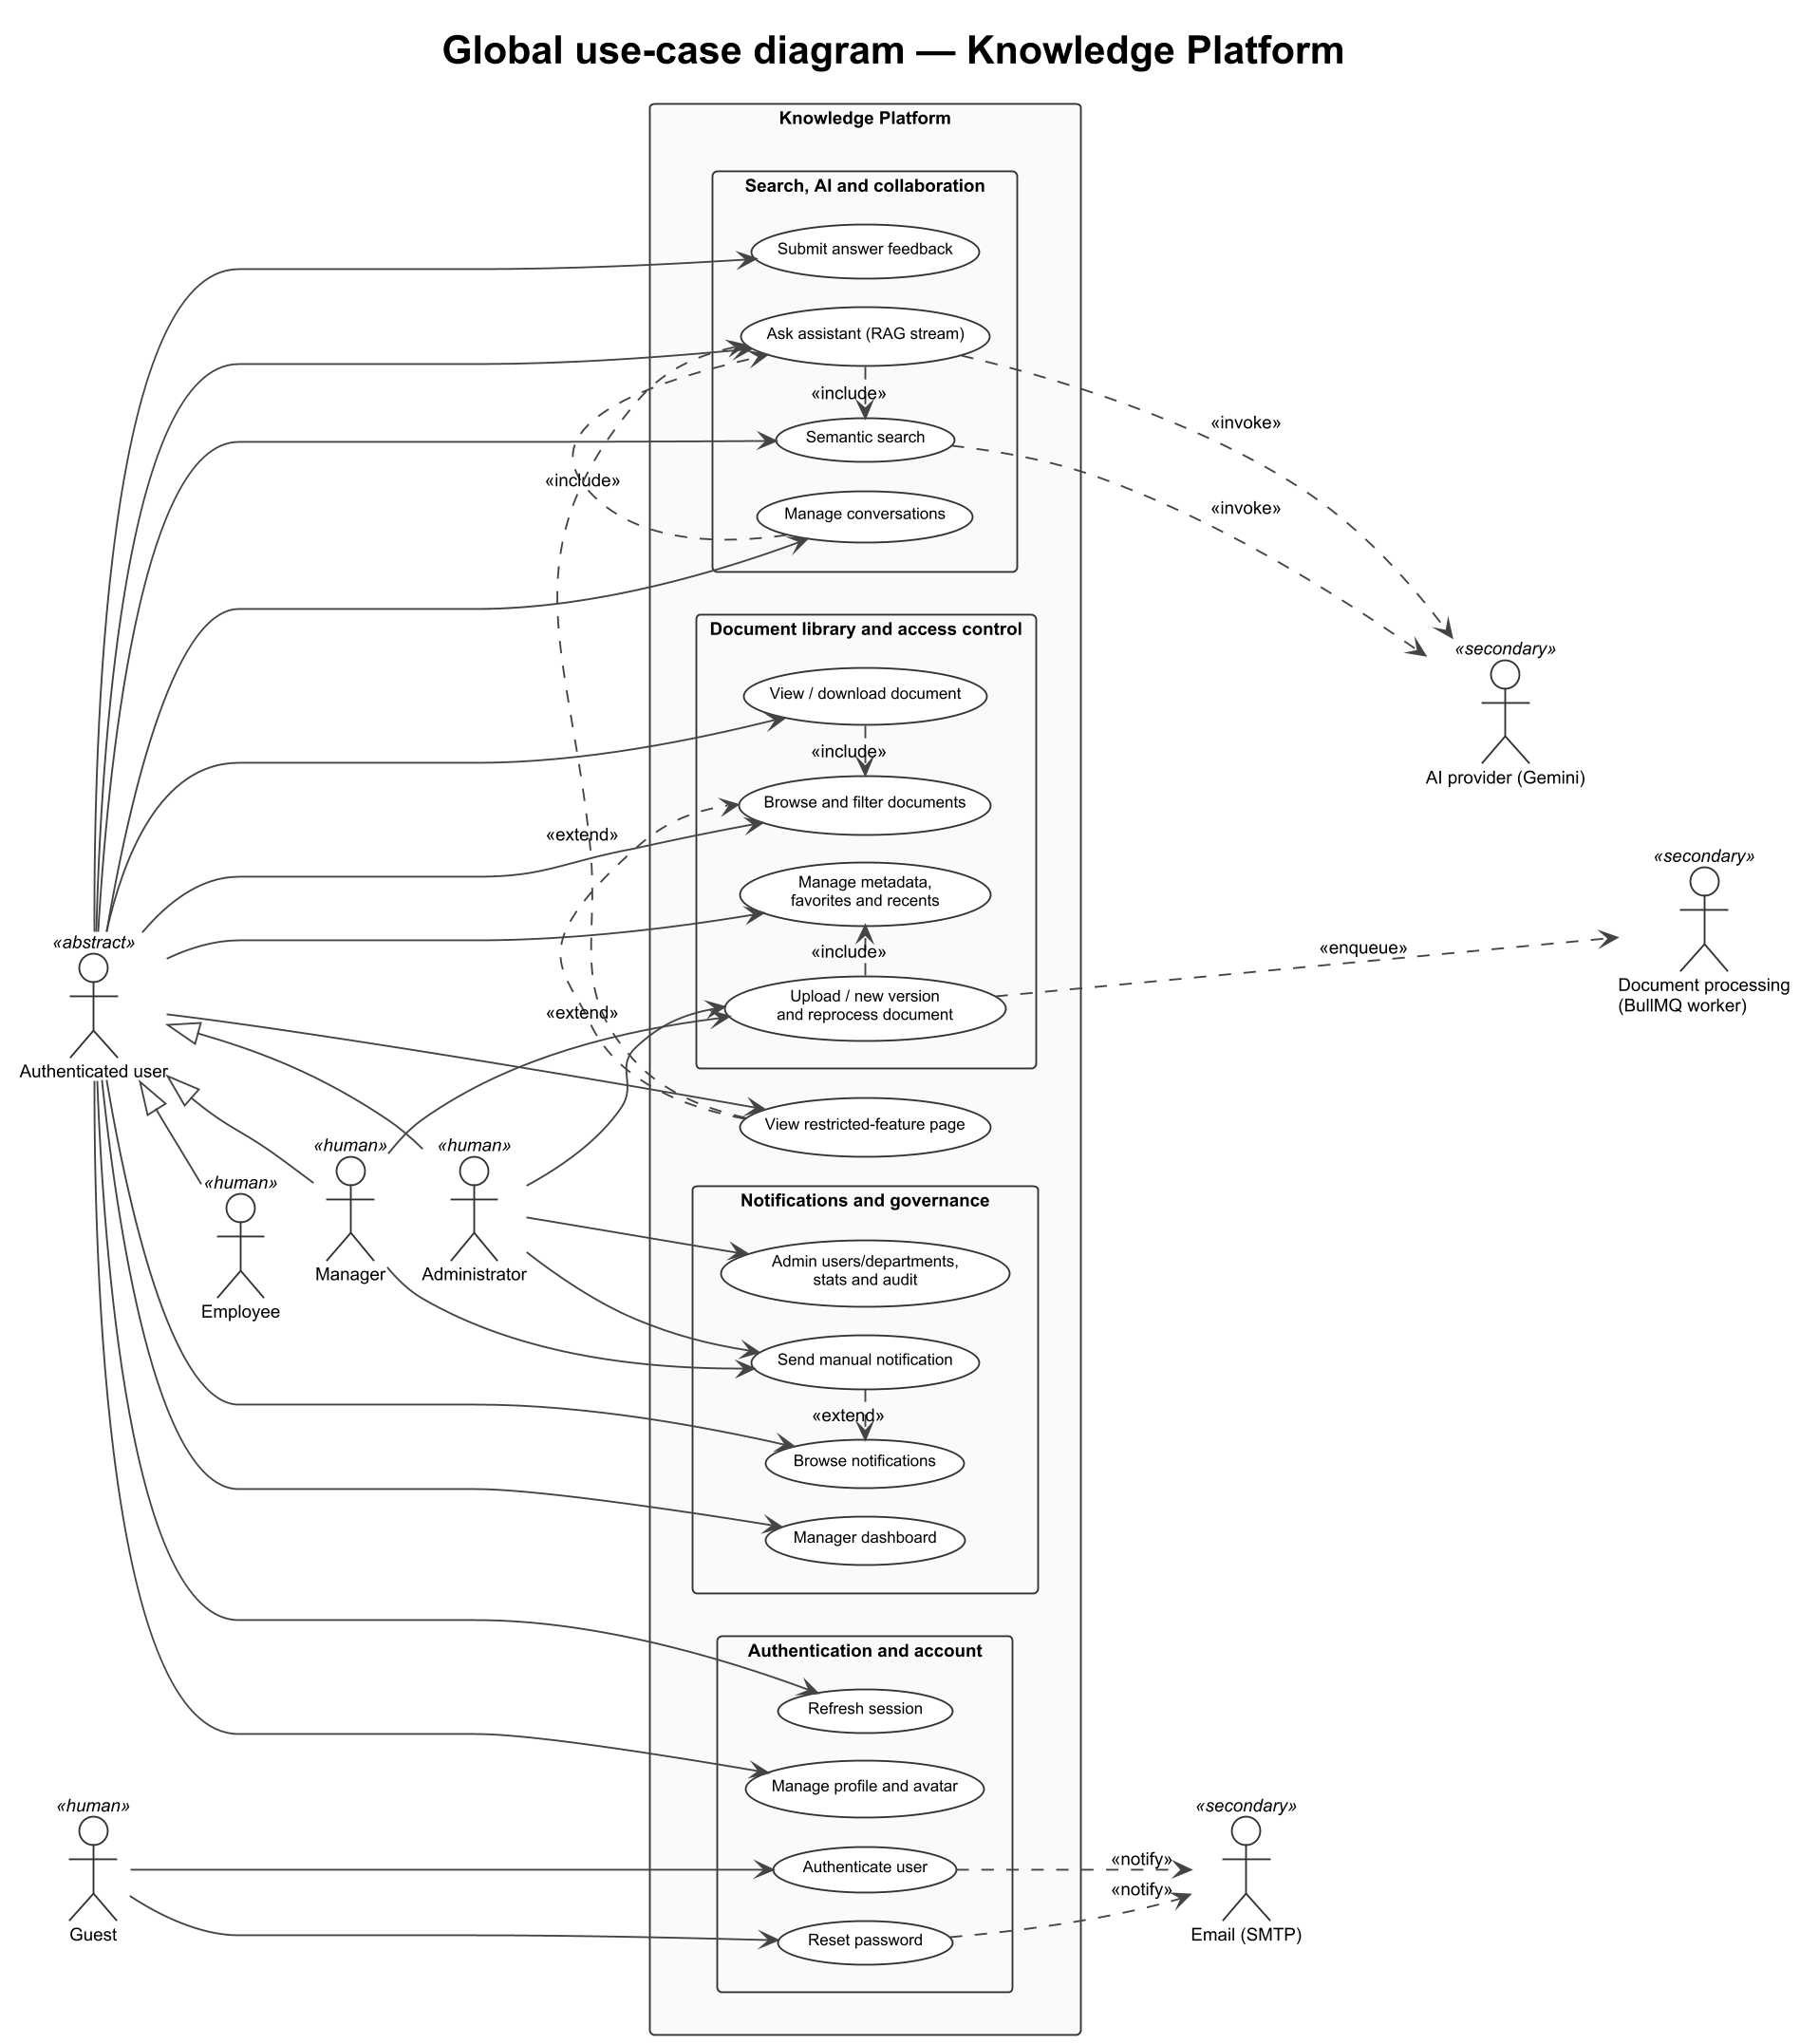
\includegraphics[width=\textwidth]{assets/figures/global-use-case-knowledge-platform.png}
  \caption{Global use-case diagram of the Knowledge Platform}
  \label{fig:use-cases}
\end{figure}

The use-case packages map directly to the functional requirement domains in
Table~\ref{tab:requirements}: authentication (FR-01, FR-02, FR-12), document
management (FR-03 to FR-05), search and AI (FR-06 to FR-08), notifications
(FR-09), and governance (FR-10, FR-11).

\section{Functional and Non-Functional Requirements}

The requirements were derived from an analysis of user workflows and system
architecture, ensuring alignment between functional needs and system design.

\subsection{Functional Requirements}

The system defines a set of functional requirements organized around
\textbf{authentication} (FR-01, FR-02), \textbf{document management} (FR-03 to
FR-05), \textbf{search and AI capabilities} (FR-06 to FR-08),
\textbf{notifications} (FR-09), \textbf{administration} (FR-10, FR-11), and
\textbf{system-level feature controls} (FR-12). Access to all functionalities is
governed by a hybrid authorization model combining Role-Based Access Control
(RBAC), Attribute-Based Access Control (ABAC), and per-user restriction flags
(see Subsection~\ref{subsec:access-control-model}).

\begin{xltabular}{\linewidth}{|>{\RaggedRight\arraybackslash}p{0.85cm}|>{\RaggedRight\arraybackslash}p{0.24\linewidth}|>{\RaggedRight\arraybackslash}p{0.31\linewidth}|Y|}
\caption{Functional requirements with acceptance criteria}
\label{tab:requirements} \\
\hline
\rowcolor{sectionblue!15}
\textbf{ID} & \textbf{Requirement} & \textbf{Acceptance criterion} & \textbf{Module / API} \\
\hline
\endfirsthead
\hline
\rowcolor{sectionblue!15}
\textbf{ID} & \textbf{Requirement} & \textbf{Acceptance criterion} & \textbf{Module / API} \\
\hline
\endhead
\hline
\endfoot

FR-01 &
JWT authentication with HttpOnly refresh cookie rotation &
Login returns access token; refresh rotates session atomically; replay revokes family &
\tcodelines{POST /auth/login}{POST /auth/refresh} \\
\hline
FR-02 &
User profile management including avatar upload &
Platform-hosted avatar served with correct CORP header; cross-origin display verified &
\tcodelines{PATCH /auth/profile}{GET /avatars/:id} \\
\hline
FR-03 &
Document upload with multi-format extraction and async ingest &
File stored on disk; ingest job enqueued; version status reaches READY &
\apicode{POST /documents/upload}\newline BullMQ worker \\
\hline
FR-04 &
Document visibility control (ALL / DEPARTMENT / PRIVATE) &
Unauthorised access returns 404 (not 403) to prevent enumeration &
\tcode{canReadDocument}\newline\tcode{documentAccess.ts} \\
\hline
FR-05 &
Document metadata: tags, favorites, recents, archive &
Tag autocomplete, favorite toggle, recent view, archive/restore all persisted &
\tcode{documents.ts} \\
\hline
FR-06 &
Semantic vector search over department-scoped document corpus &
Vector similarity results ranked correctly; access-filtered; respects restrictions &
\apicode{POST /search/semantic} \\
\hline
FR-07 &
Hybrid RAG Ask with SSE streaming and source citations &
SSE events emitted in order: \tcode{sources}, \tcode{token}, \tcode{done}; citations reference real chunks &
\tcodelines{POST /search/ask}{ragCompletion.ts} \\
\hline
FR-08 &
Conversation history with per-message feedback &
Threads persisted; thumbs up/down stored; feedback stats available to admin &
\apicode{/conversations/*} \\
\hline
FR-09 &
Automatic and manual notification system with attachments &
Department-scoped events emitted on document create/update/delete; manual send available to managers/admins &
\tcodelines{/notifications/*}{notificationService.ts} \\
\hline
FR-10 &
Full administrative control: user/department CRUD, bulk operations, audit &
Last-admin safety enforced; CSV imports escaped; audit log exportable &
\apicode{/admin/*} \\
\hline
FR-11 &
Manager dashboard scoped to manageable departments &
Only departments from \tcode{manageable\-DepartmentIds} returned; member list correct &
\apicode{/manager/*} \\
\hline
FR-12 &
Per-user feature restriction flags &
Flags block login, document access, and AI queries via middleware; restricted page displayed &
\tcode{requireDoc\-LibraryAccess}\newline\tcode{requireUse\-AiQueries} \\
\hline
\end{xltabular}

Table~\ref{tab:fr-traceability} summarises the mapping from each functional
requirement to its primary implementation module and development sprint.

\begin{table}[H]
\centering
\caption{Functional requirements traceability summary}
\label{tab:fr-traceability}
\renewcommand{\arraystretch}{1.35}
\begin{tabularx}{\textwidth}{|>{\RaggedRight\arraybackslash}p{0.85cm}|>{\RaggedRight\arraybackslash}p{2.6cm}|Y|>{\Centering\arraybackslash}p{1.0cm}|}
\hline
\rowcolor{sectionblue!15}
\textbf{ID} & \textbf{Domain} & \textbf{Primary module / service} & \textbf{Sprint} \\
\hline
FR-01 & Authentication & \tcode{auth.ts} (JWT, refresh families) & S1 \\
\hline
FR-02 & Profile management & \tcode{auth.ts}, \tcode{avatarsPublic.ts} & S1 \\
\hline
FR-03 & Document ingest & BullMQ ingest worker, \tcode{documents.ts} & S2 \\
\hline
FR-04 & Access control & \tcode{documentAccess.ts}, visibility filters & S2 \\
\hline
FR-05 & Document organisation & \tcode{documents.ts} (tags, favorites, archive) & S2 \\
\hline
FR-06 & Semantic search & \tcode{search.ts}, pgvector retrieval & S3 \\
\hline
FR-07 & RAG question answering & \tcode{ragCompletion.ts} (hybrid RAG pipeline) & S3 \\
\hline
FR-08 & Conversations & \tcode{conversations.ts} & S3 \\
\hline
FR-09 & Notifications & \tcode{notificationService.ts}, \tcode{notifications.ts} & S4 \\
\hline
FR-10 & Administration & \tcode{admin.ts} & S4 \\
\hline
FR-11 & Manager dashboard & \tcode{manager.ts} & S4 \\
\hline
FR-12 & Feature restrictions & Auth middleware, \tcode{requireUseAiQueries} & S1 \\
\hline
\end{tabularx}
\end{table}

Chapter~\ref{ch:architecture} extends this summary with design elements and
validation test references (Table~\ref{tab:traceability-main}).

\subsection{Non-Functional Requirements}

\begin{table}[H]
\centering
\caption{Non-functional requirements}
\label{tab:nfr}
\renewcommand{\arraystretch}{1.4}
\begin{tabularx}{\textwidth}{|>{\RaggedRight\arraybackslash}p{0.85cm}|>{\RaggedRight\arraybackslash}p{0.38\linewidth}|Y|}
\hline
\rowcolor{sectionblue!15}
\textbf{ID} & \textbf{Requirement} & \textbf{Acceptance criterion} \\
\hline
NFR-01 & Health monitoring endpoint &
\tcode{GET /health} returns \tcode{200 \{status: "ok"\}} when PostgreSQL and Redis
are reachable; \tcode{503} with per-check detail otherwise \\
\hline
NFR-02 & Security headers and rate limiting &
Helmet CSP enforced on all responses; login limited to 15 req/15 min/IP; Ask
limited to 12 req/min/IP \\
\hline
NFR-03 & Single-flight refresh token (web client) &
Parallel requests from the same tab do not trigger multiple \tcode{/auth/refresh}
calls; the in-flight promise is shared \\
\hline
NFR-04 & Docker Compose reproducibility &
\tcode{docker compose up -{}-build} starts all four services (postgres, redis, api,
web) in a healthy state; migrations run automatically \\
\hline
NFR-05 & Integration test coverage &
All Vitest/Supertest suites pass on a real PostgreSQL + Redis instance with seeded
data \\
\hline
NFR-06 & RAG evaluation harness &
\tcode{npm run eval:rag:quick} executes without error and writes a JSON report
to \tcode{eval-reports/} \\
\hline
\end{tabularx}
\end{table}

\subsection{Access Control Model}
\label{subsec:access-control-model}

Building on the RBAC concepts introduced in Chapter~\ref{ch:state-of-the-art},
the platform enforces a \textbf{hybrid authorization model} that operates at three
complementary layers. This subsection specifies how the theoretical foundations are
applied to the requirements defined above.

\begin{itemize}
  \item \textbf{Role-Based Access Control (RBAC)}: every user holds one platform
    role --- \texttt{ADMIN}, \texttt{MANAGER}, or \texttt{EMPLOYEE} --- that
    determines coarse-grained capabilities. Administrators manage users,
    departments, and platform configuration (FR-10); managers access
    department-scoped dashboards and announcements (FR-11); employees use the
    document library, search, and AI assistant within their permitted scope.
  \item \textbf{Attribute-Based Access Control (ABAC)}: permissions are further
    constrained by attributes such as department membership and document
    visibility (\texttt{ALL}, \texttt{DEPARTMENT}, \texttt{PRIVATE}). Retrieval
    and RAG pipelines apply these filters before returning results, ensuring that
    semantic search and generated answers never expose unauthorised content
    (FR-04, FR-06, FR-07).
  \item \textbf{Per-user feature restriction flags}: administrators can disable
    specific capabilities for individual users --- for example, blocking document
    library access or AI queries --- via middleware that intercepts requests
    before business logic executes (FR-12).
\end{itemize}

This layered model ensures fine-grained control over system capabilities while
maintaining scalability and security across authentication, document management,
search, and AI workflows.

\section{Specifications and Performance Indicators}

The following Key Performance Indicators (KPIs) link requirements to the validation
chapter (Chapter~\ref{ch:validation}):

\begin{table}[H]
\centering
\caption{Key performance indicators}
\label{tab:kpis}
\renewcommand{\arraystretch}{1.4}
\begin{tabularx}{\textwidth}{|>{\RaggedRight\arraybackslash}p{2.5cm}|Y|>{\RaggedRight\arraybackslash}p{2.0cm}|}
\hline
\rowcolor{sectionblue!15}
\textbf{KPI} & \textbf{Measurement method} & \textbf{Target} \\
\hline
Ingest reliability &
Percentage of uploaded documents reaching \tcode{READY} status without
\tcode{FAILED} &
$\geq 95\%$ \\
\hline
Integration test pass rate &
\tcode{npm run test:api} output: passed / total &
74 / 74 (100\%) \\
\hline
RAG topic classification (no API key) &
\tcode{eval:rag:quick} optimizer pass rate &
$\geq 15/34$ (degraded mode) \\
\hline
RAG judge scores (with API key) &
Faithfulness and relevance from automated judge &
Documented in eval report \\
\hline
Security: refresh replay &
Reuse of rotated token triggers family revocation &
Verified by auth test suite \\
\hline
Security: avatar CORP &
\tcode{Cross-Origin-Resource-Policy: cross-origin} header present on avatar responses &
Verified by avatars test \\
\hline
\end{tabularx}
\end{table}

\section{Selected Methodology}

\subsection{Agile Scrum Framework}

The project was managed using the \textbf{Agile Scrum} methodology, chosen for its
iterative structure, its emphasis on working deliverables at the end of each sprint,
and its adaptability to evolving requirements — all well-suited to a complex full-stack
product developed by a single engineer over a bounded internship period.

\subsubsection{Scrum Roles}

\begin{itemize}
  \item \textbf{Product Owner}: \IndustrialSupervisor{} (\CompanyName), responsible
    for validating feature priorities and acceptance criteria.
  \item \textbf{Scrum Master / Developer}: \StudentName, responsible for sprint
    planning, execution, daily self-review, and retrospective.
  \item \textbf{Academic Advisor}: \AcademicSupervisor{} (ESPRIM), providing
    methodological and scientific guidance at sprint boundaries.
\end{itemize}

\subsubsection{Scrum Artefacts}

\begin{itemize}
  \item \textbf{Product Backlog}: the complete list of functional and non-functional
    requirements (FR-01 to FR-12, NFR-01 to NFR-06) prioritised by business value
    and technical dependency.
  \item \textbf{Sprint Backlog}: the subset of backlog items committed to in each
    sprint, decomposed into implementation tasks.
  \item \textbf{Increment}: a working, tested vertical slice of the platform delivered
    at the end of each sprint.
  \item \textbf{Definition of Done}: a requirement is considered done when (a) the
    feature is implemented, (b) at least one integration test covers the happy path
    and one error path, and (c) the corresponding API route or module is manually
    validated.
\end{itemize}

\subsubsection{Sprint Structure}

Each sprint followed a fixed rhythm:

\begin{enumerate}
  \item \textbf{Sprint Planning}: review backlog, select items, decompose into tasks,
    estimate effort.
  \item \textbf{Development}: implement features, write integration tests, perform
    code review against security and style guidelines.
  \item \textbf{Sprint Review}: demonstrate the working increment; validate against
    acceptance criteria.
  \item \textbf{Sprint Retrospective}: identify what worked, what blocked, and what
    to improve in the next sprint.
\end{enumerate}

\subsection{Sprint Plan}

The project was structured across \textbf{five sprints}, each delivering a coherent
and independently testable platform capability. Detailed interaction design for each
sprint appears in Section~\ref{sec:sprint-design} of Chapter~\ref{ch:architecture}.

\begin{table}[H]
\centering
\caption{Agile Scrum sprint plan}
\label{tab:sprints}
\footnotesize
\renewcommand{\arraystretch}{1.3}
\setlength{\tabcolsep}{2.5pt}
\begin{tabularx}{\linewidth}{|>{\Centering\arraybackslash}p{0.055\linewidth}|>{\RaggedRight\arraybackslash}p{0.16\linewidth}|>{\RaggedRight\arraybackslash}X|>{\RaggedRight\arraybackslash}p{0.13\linewidth}|>{\Centering\arraybackslash}p{0.055\linewidth}|}
\hline
\rowcolor{sectionblue!15}
\textbf{Spr.} & \textbf{Theme} & \textbf{Deliverables} & \textbf{Req.} & \textbf{Des.} \\
\hline
\textbf{S1} &
Auth., users, RBAC &
JWT login/logout/refresh (HttpOnly cookies), refresh-token family revocation,
password policy, session cap, per-user restrictions, profile/avatar, RBAC middleware &
FR-01, FR-02, FR-12 \newline NFR-02, NFR-03 &
\ref{subsec:sprint1-design} \\
\hline
\textbf{S2} &
Document library \& ingest &
Multi-format upload (PDF, Office, HTML, XML, ZIP), BullMQ worker
(extract$\to$chunk$\to$embed$\to$persist), versioning, tags, favorites, recents,
archive, visibility, audit log &
FR-03, FR-04, FR-05 &
\ref{subsec:sprint2-design} \\
\hline
\textbf{S3} &
Hybrid RAG \& Ask &
Query optimiser, hybrid retrieval (pgvector + BM25 + RRF), LLM reranking,
neighbour expansion, SSE answers with citations, confidence scoring, critique,
claim verification, follow-ups, feedback loop, conversations &
FR-06, FR-07, FR-08 \newline NFR-06 &
\ref{subsec:sprint3-design} \\
\hline
\textbf{S4} &
Admin, manager, notifications &
Admin CRUD (users, departments, merge, bulk ops, CSV), dept-access management,
KPI dashboard, activity/audit exports, manager view, auto/manual notifications &
FR-09, FR-10, FR-11 &
\ref{subsec:sprint4-design} \\
\hline
\textbf{S5} &
Tests, eval \& deploy &
74 Vitest/Supertest integration tests, RAG eval CLI (automated judge),
Docker Compose prod config, migration pipeline, 54 UML diagrams, README &
NFR-01, NFR-04, NFR-05 \newline NFR-06 &
\ref{subsec:sprint5-design} \\
\hline
\end{tabularx}
\end{table}

The \textbf{Des.} column references the sprint interaction-design subsections of
Section~\ref{sec:sprint-design} (Chapter~\ref{ch:architecture}).

\subsubsection{Sprint Timeline}
\label{subsec:sprint-timeline}

Figure~\ref{fig:scrum-timeline} illustrates the sprint sequence defined in
Table~\ref{tab:sprints} and the iterative delivery of working increments across
the project duration. Each sprint builds on the previous one: authentication
and access control (S1), document corpus (S2), hybrid RAG (S3), governance
(S4), then operational hardening and validation (S5).

\begin{figure}[H]
\centering
\begin{tikzpicture}[
  sprint/.style={draw, fill=sectionblue!20, rounded corners, minimum width=2.8cm,
                 minimum height=1.2cm, align=center, font=\small},
  arrow/.style={->, thick, color=sectionblue}
]
\node[sprint] (s1) at (0,0)    {\textbf{Sprint 1}\\\small Auth \& RBAC};
\node[sprint] (s2) at (3.2,0)  {\textbf{Sprint 2}\\\small Documents};
\node[sprint] (s3) at (6.4,0)  {\textbf{Sprint 3}\\\small RAG Engine};
\node[sprint] (s4) at (9.6,0)  {\textbf{Sprint 4}\\\small Admin};
\node[sprint] (s5) at (12.8,0) {\textbf{Sprint 5}\\\small Testing};
\draw[arrow] (s1) -- (s2);
\draw[arrow] (s2) -- (s3);
\draw[arrow] (s3) -- (s4);
\draw[arrow] (s4) -- (s5);
\end{tikzpicture}
\caption{Scrum sprint timeline — iterative delivery across five sprints}
\label{fig:scrum-timeline}
\end{figure}

\subsubsection{Sprint Backlogs}

Tables~\ref{tab:s1-backlog}--\ref{tab:s5-backlog} detail each sprint backlog at
user-story level. The stories refine the scope presented in Table~\ref{tab:sprints}
and provide planning-level traceability between implementation tasks, acceptance
criteria, and effort estimation. Interaction flows for every story are documented
in Section~\ref{sec:sprint-design}.

\paragraph{Sprint 1 --- Authentication and access control.}

\begin{table}[H]
\centering
\caption{Sprint 1 backlog: authentication and access control}
\label{tab:s1-backlog}
\footnotesize
\renewcommand{\arraystretch}{1.3}
\setlength{\tabcolsep}{2.5pt}
\begin{tabularx}{\linewidth}{|>{\RaggedRight\arraybackslash}p{0.09\linewidth}|>{\RaggedRight\arraybackslash}X|>{\RaggedRight\arraybackslash}p{0.33\linewidth}|>{\Centering\arraybackslash}p{0.045\linewidth}|>{\Centering\arraybackslash}p{0.08\linewidth}|}
\hline
\rowcolor{sectionblue!15}
\textbf{ID} & \textbf{User Story} & \textbf{Acceptance Criteria} & \textbf{SP} & \textbf{Pri.} \\
\hline
US-S1-01 &
As a guest, I want to sign in securely so that I can access authorised platform features. &
\tcode{POST /auth/login} issues access token + refresh cookie; invalid credentials rejected; login limiter enforced. &
5 & High \\
\hline
US-S1-02 &
As an authenticated user, I want seamless session continuity so that refresh operations are secure and race-condition free. &
\tcode{/auth/refresh} rotates token family atomically; replay revokes family; single-flight refresh on web client. &
8 & High \\
\hline
US-S1-03 &
As an authenticated user, I want to sign out so that active refresh sessions are revoked. &
Logout revokes current refresh session; subsequent refresh attempts fail. &
2 & Med. \\
\hline
US-S1-04 &
As a user, I want to view and update my profile, including avatar, so that my account information remains accurate. &
\tcode{PATCH /auth/profile} persists updates; avatar upload works; avatar route serves CORP header for cross-origin display. &
5 & High \\
\hline
US-S1-05 &
As an administrator, I want role-based and per-user access restrictions so that capabilities can be controlled precisely. &
Role middleware enforces ADMIN/MANAGER/EMPLOYEE boundaries; restriction flags block protected features and redirect to restricted page. &
8 & High \\
\hline
US-S1-06 &
As a security owner, I want baseline HTTP protections so that authentication endpoints resist abuse. &
Helmet headers active globally; login and Ask endpoints rate-limited according to configured thresholds. &
3 & Med. \\
\hline
\end{tabularx}
\end{table}

\paragraph{Sprint 2 --- Document library and ingest.}

\begin{table}[H]
\centering
\caption{Sprint 2 backlog: document library and ingest}
\label{tab:s2-backlog}
\footnotesize
\renewcommand{\arraystretch}{1.3}
\setlength{\tabcolsep}{2.5pt}
\begin{tabularx}{\linewidth}{|>{\RaggedRight\arraybackslash}p{0.09\linewidth}|>{\RaggedRight\arraybackslash}X|>{\RaggedRight\arraybackslash}p{0.33\linewidth}|>{\Centering\arraybackslash}p{0.045\linewidth}|>{\Centering\arraybackslash}p{0.08\linewidth}|}
\hline
\rowcolor{sectionblue!15}
\textbf{ID} & \textbf{User Story} & \textbf{Acceptance Criteria} & \textbf{SP} & \textbf{Pri.} \\
\hline
US-S2-01 &
As an employee, I want to upload documents in common formats so that they enter the shared library. &
\apicode{POST /documents/upload} validates MIME/size, stores file on disk, creates version row, enqueues ingest job. &
8 & High \\
\hline
US-S2-02 &
As the system, I want to ingest uploaded files asynchronously so that text is searchable and embeddable. &
BullMQ worker extracts text, chunks content, computes 768-d embeddings, persists \tcode{Chunk} rows; version reaches \tcode{READY}. &
13 & High \\
\hline
US-S2-03 &
As a security owner, I want visibility rules enforced so that unauthorised users cannot discover restricted documents. &
\tcode{ALL}/\tcode{DEPARTMENT}/\tcode{PRIVATE} enforced via \tcode{canReadDocument}; unauthorised access returns 404. &
8 & High \\
\hline
US-S2-04 &
As an employee, I want to browse, search, and open documents so that I can find relevant files quickly. &
\apicode{GET /documents} supports filters/pagination; \apicode{GET /documents/:id} returns metadata and active version; download streams file bytes. &
5 & High \\
\hline
US-S2-05 &
As an employee, I want favorites and recents so that I can return to frequently used documents. &
Favorite toggle and recent-view endpoints persist per user; library home surfaces both lists. &
3 & Med. \\
\hline
US-S2-06 &
As a document owner, I want versioning and re-ingestion so that updates and embedding upgrades are supported. &
\apicode{POST /documents/:id/versions} creates new version + ingest job; \apicode{POST .../reprocess} forces re-ingest of existing version. &
8 & Med. \\
\hline
US-S2-07 &
As a manager, I want to update metadata and retain an audit trail so that document governance is traceable. &
\apicode{PATCH /documents/:id} updates title, tags, visibility within scope; changes recorded in per-document audit log. &
5 & Med. \\
\hline
\end{tabularx}
\end{table}

\paragraph{Sprint 3 --- Search, RAG and conversations.}

\begin{table}[H]
\centering
\caption{Sprint 3 backlog: search, RAG and conversations}
\label{tab:s3-backlog}
\footnotesize
\renewcommand{\arraystretch}{1.3}
\setlength{\tabcolsep}{2.5pt}
\begin{tabularx}{\linewidth}{|>{\RaggedRight\arraybackslash}p{0.09\linewidth}|>{\RaggedRight\arraybackslash}X|>{\RaggedRight\arraybackslash}p{0.33\linewidth}|>{\Centering\arraybackslash}p{0.045\linewidth}|>{\Centering\arraybackslash}p{0.08\linewidth}|}
\hline
\rowcolor{sectionblue!15}
\textbf{ID} & \textbf{User Story} & \textbf{Acceptance Criteria} & \textbf{SP} & \textbf{Pri.} \\
\hline
US-S3-01 &
As an employee, I want semantic search over the corpus so that I can find relevant passages by meaning. &
\apicode{POST /search/semantic} embeds query, ranks department-scoped chunks via pgvector, returns snippet previews. &
8 & High \\
\hline
US-S3-02 &
As an employee, I want cited answers streamed in real time so that I receive grounded responses to natural-language questions. &
\apicode{POST /search/ask} runs hybrid retrieval + RRF + rerank; SSE emits \tcode{sources}, \tcode{token}, \tcode{done} with chunk citations. &
13 & High \\
\hline
US-S3-03 &
As an employee, I want persistent conversation threads so that I can review prior questions and answers. &
\apicode{/conversations} supports create, list, rename, delete; messages store sources, confidence, and citations. &
8 & High \\
\hline
US-S3-04 &
As an employee, I want to rate assistant answers so that poor responses can be identified and improved. &
\apicode{POST .../feedback} stores thumbs up/down; admin stats endpoint aggregates sentiment and volume. &
5 & Med. \\
\hline
US-S3-05 &
As a data scientist, I want a reproducible RAG evaluation harness so that retrieval quality can be measured over time. &
\tcode{npm run eval:rag:quick} and \tcode{eval:rag} write JSON reports under \tcode{eval-reports/} without breaking CI. &
8 & Med. \\
\hline
\end{tabularx}
\end{table}

\paragraph{Sprint 4 --- Governance and notifications.}

\begin{table}[H]
\centering
\caption{Sprint 4 backlog: governance and notifications}
\label{tab:s4-backlog}
\footnotesize
\renewcommand{\arraystretch}{1.3}
\setlength{\tabcolsep}{2.5pt}
\begin{tabularx}{\linewidth}{|>{\RaggedRight\arraybackslash}p{0.09\linewidth}|>{\RaggedRight\arraybackslash}X|>{\RaggedRight\arraybackslash}p{0.33\linewidth}|>{\Centering\arraybackslash}p{0.045\linewidth}|>{\Centering\arraybackslash}p{0.08\linewidth}|}
\hline
\rowcolor{sectionblue!15}
\textbf{ID} & \textbf{User Story} & \textbf{Acceptance Criteria} & \textbf{SP} & \textbf{Pri.} \\
\hline
US-S4-01 &
As an employee, I want automatic notifications on document events so that I stay informed of library changes. &
Document create/update/delete emits department-scoped inbox entries via \tcode{notificationService.ts}. &
5 & High \\
\hline
US-S4-02 &
As a manager or admin, I want to send manual announcements so that I can communicate with targeted teams. &
\apicode{POST /notifications/send} validates audience scope; optional attachments downloadable by recipients. &
5 & High \\
\hline
US-S4-03 &
As an employee, I want a notification inbox so that I can read and dismiss messages. &
List, unread count, mark-read, and mark-all-read endpoints; web client polls with badge indicator. &
5 & Med. \\
\hline
US-S4-04 &
As a manager, I want a department dashboard so that I can oversee teams and documents I manage. &
\apicode{/manager/*} returns only \tcode{manageableDepartmentIds}; member lists and department documents scoped correctly. &
8 & High \\
\hline
US-S4-05 &
As an administrator, I want full user and department administration so that the platform reflects organisational structure. &
\apicode{/admin/*} supports user CRUD, department create/merge, last-admin safety, CSV import with formula escaping. &
13 & High \\
\hline
US-S4-06 &
As an administrator, I want bulk access management and operational exports so that governance tasks scale efficiently. &
Bulk department-access PUT, KPI stats, activity log, document audit, and CSV exports available to admins. &
8 & Med. \\
\hline
\end{tabularx}
\end{table}

\paragraph{Sprint 5 --- Operations, testing and deployment.}

\begin{table}[H]
\centering
\caption{Sprint 5 backlog: operations, testing and deployment}
\label{tab:s5-backlog}
\footnotesize
\renewcommand{\arraystretch}{1.3}
\setlength{\tabcolsep}{2.5pt}
\begin{tabularx}{\linewidth}{|>{\RaggedRight\arraybackslash}p{0.09\linewidth}|>{\RaggedRight\arraybackslash}X|>{\RaggedRight\arraybackslash}p{0.33\linewidth}|>{\Centering\arraybackslash}p{0.045\linewidth}|>{\Centering\arraybackslash}p{0.08\linewidth}|}
\hline
\rowcolor{sectionblue!15}
\textbf{ID} & \textbf{User Story} & \textbf{Acceptance Criteria} & \textbf{SP} & \textbf{Pri.} \\
\hline
US-S5-01 &
As an operator, I want a health endpoint so that I can verify database and queue connectivity. &
\apicode{GET /health} returns \tcode{200} when PostgreSQL and Redis are reachable; \tcode{503} with per-check detail otherwise. &
3 & High \\
\hline
US-S5-02 &
As a developer, I want automated integration tests so that regressions are caught before release. &
\tcode{npm run test:api} runs 74 Vitest/Supertest cases across 10 suites on real DB/Redis; target 100\% pass. &
13 & High \\
\hline
US-S5-03 &
As an operator, I want reproducible containerised deployment so that the platform can be started consistently. &
\tcode{docker compose up -{}-build} starts postgres, redis, api, web healthy; migrations run automatically. &
8 & High \\
\hline
US-S5-04 &
As a data scientist, I want automated RAG judge evaluation so that answer quality can be tracked with an API key. &
\tcode{npm run eval:rag} produces faithfulness/relevance scores in \tcode{eval-reports/}; quick mode runs without key. &
8 & Med. \\
\hline
US-S5-05 &
As a maintainer, I want complete design documentation so that the system is defensible and maintainable. &
54 PlantUML diagrams exported; README and architecture guide updated; sequence flows indexed in Appendix~\ref{annex:diagrams}. &
5 & Med. \\
\hline
\end{tabularx}
\end{table}

\subsection{Development and Modelling Tools}

\begin{table}[H]
\centering
\caption{Development and modelling tools}
\renewcommand{\arraystretch}{1.3}
\begin{tabularx}{\textwidth}{|>{\RaggedRight\arraybackslash}p{3.2cm}|Y|}
\hline
\rowcolor{sectionblue!15}
\textbf{Tool} & \textbf{Usage in project} \\
\hline
Prisma Schema DSL & Domain modelling and 29 sequential migrations \\
\hline
PlantUML & 54 UML diagrams (3 structural, 5 sprint use-case, 5 sprint class, 41 sequence) \\
\hline
Vitest + Supertest & Integration testing across all API domains \\
\hline
Docker Compose & Reproducible dev and production environment \\
\hline
GitHub Actions & CI pipeline (lint, audit, typecheck, integration tests) \\
\hline
Zod & Runtime request validation for all API inputs \\
\hline
\end{tabularx}
\end{table}

\subsection{Data Science Orientation}

In alignment with the Data Science discipline, the following elements of the project
are treated as data-science artefacts:

\begin{itemize}
  \item \textbf{Corpus and embeddings}: the set of ingested documents and their
    768-dimensional vector representations in PostgreSQL constitute the experimental
    dataset on which retrieval quality is measured.
  \item \textbf{Query optimisation}: classifying query type (factual, summary,
    comparative, procedural, out-of-scope) and rewriting queries for retrieval is
    analogous to feature engineering in a machine learning pipeline.
  \item \textbf{RRF ensemble}: the weighted fusion of dense and sparse retrieval
    results is an ensemble method with tunable hyperparameters (\texttt{RRF\_K},
    \texttt{RRF\_DENSE\_WEIGHT}, \texttt{RRF\_SPARSE\_WEIGHT}).
  \item \textbf{Automated judge evaluation}: the RAG evaluation harness uses an
    LLM-as-judge to measure faithfulness, answer relevance, and context precision,
    producing reproducible JSON reports — a standard experimental validation
    workflow for generative AI systems \cite{es2024rag-eval}.
  \item \textbf{Feedback-driven adaptation}: negative user ratings are semantically
    compared to new questions using embedding cosine similarity, constituting an
    online adaptation mechanism without model retraining.
\end{itemize}

\section{Chapter Conclusion}

This chapter translated the state-of-the-art insights into a verifiable
specification by defining functional and non-functional requirements, acceptance
criteria, and requirement-to-module traceability. It also formalized the project
methodology through a five-sprint Scrum plan and detailed sprint backlogs,
linking planning artefacts to implementation and validation objectives.
Chapter~\ref{ch:architecture} presents the resulting system design, including
sprint-aligned interaction diagrams in Section~\ref{sec:sprint-design}.
